\section{Model generalisation}

\Cref{fig:imm} illustrates a probabilistic graphical representation of the IMM.\@

\begin{figure}[htbp]
\centering
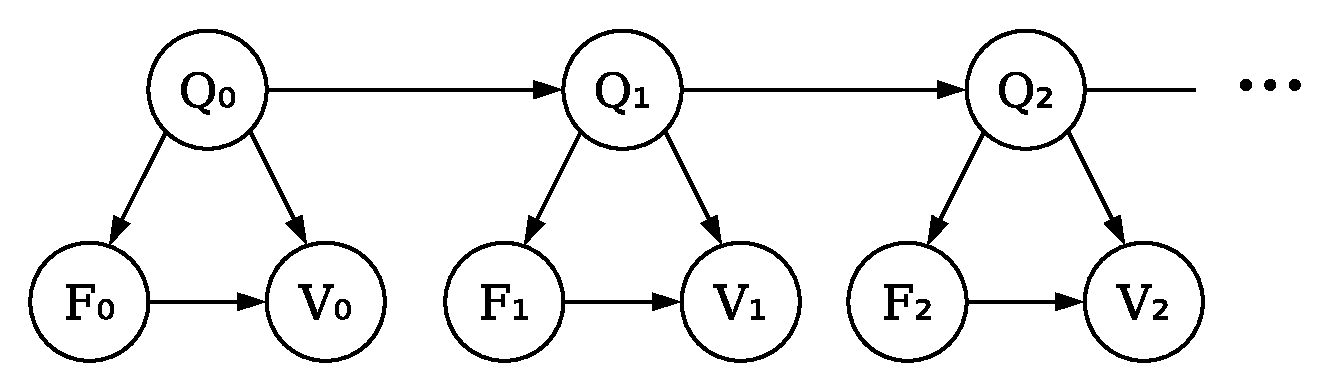
\includegraphics[width=.45\linewidth]{figure/imm}
\caption{Invisible Markov model.}%
\label{fig:imm}
\end{figure}

\newpage
\newpage

\begin{sidewaysfigure}[ht]
    \centering
    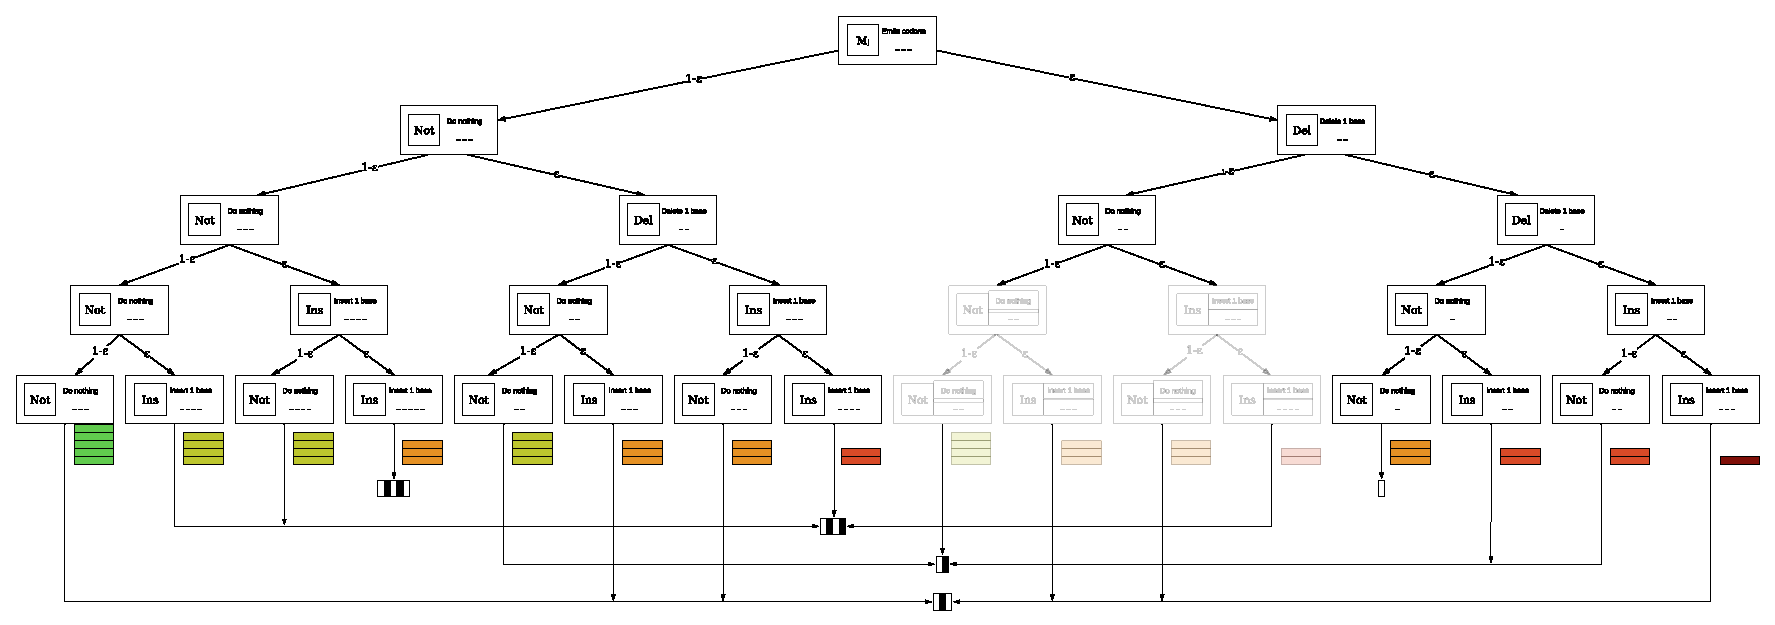
\includegraphics[scale=0.9]{figure/codon-hmm-tree}
    \caption{Matched codon HMM tree.
        The $\eps$-transitions occur infrequently and exist to account for sequence errors.
        The most probably path ends at the first leaf-node from left to right.}\label{fig:codon-hmm-tree}
\end{sidewaysfigure}
